
\documentclass[11pt,letterpaper]{article}
\usepackage[english]{babel}
%\usepackage[ansinew]{inputenc}
\usepackage[utf8]{inputenc}
% \usepackage[latin1]{inputenc}
\usepackage[letterpaper,includeheadfoot, top=0.5cm, bottom=3.0cm, right=2.0cm, left=2.0cm]{geometry}
\renewcommand{\familydefault}{\sfdefault}

\usepackage{graphicx}
\usepackage{color}
\usepackage{hyperref}
\usepackage{amssymb}
\usepackage{url}
%\usepackage{pdfpages}
\usepackage{fancyhdr}
\usepackage{hyperref}
\usepackage{subfig}
\usepackage{listings}

\usepackage{listings} %Codigo
\lstset{language=C, tabsize=4,framexleftmargin=5mm,breaklines=true}

\newcommand*{\addheight}[2][.5ex]{%
  \raisebox{0pt}[\dimexpr\height+(#1)\relax]{#2}%
}

\begin{document}
\lstset{language=SQL}
%\begin{sf}
% --------------- ---------PORTADA --------------------------------------------
\newpage
%-------------------- CABECERA ---------------------
 
\includegraphics[scale=0.9]{img/logo.png}
%------------------ TÍTULO -----------------------
\vspace*{7cm}
\begin{center}
%\huge {Título Medio}\\
%\vspace{1cm}
\Large{CS5785 Applied Machine Learning - Fall 2017} \\
\vspace{3mm}
\huge{Homework 1}
\end{center}

%------------------ INFO -----------------------
\vfill
\begin{flushright}
\begin{minipage}{.45\linewidth}
\textbf{Team:} \hspace{5.5em} Navdeep Singh\\
\textcolor{white}{.} \hspace{8.1em} Vicente Rotman\\
\textbf{Professor:} \hspace{3.9em} Sergie Belongie\\
\textbf{Date:} \hspace{6.2em}18-10-2015 
\end{minipage}
\end{flushright}
\newpage


% ------------RESUMEN----------------------
\section{DigitRecognizer}
After downloaded the data from Digit Recognizer competition on Kaggle. Start working on the python code in the file named \textbf{digit\_recognizer.py}. The function called \textbf{main} open the file, it could be the test or train data and store all the data in 2 python lists. One called \textbf{labels\_test\_data} that has the labels of each digit and another called \textbf{test\_data} that stores the digits in the same order as the labels.
\subsection{b) Write a function to display an MNIST digit. Display one of each digit}
For this part there are 2 functions involved. The first one called \textbf{getOneSampleOfEachDigit(labels, data)} which returns a list with 10 digits, one of each option from 0 - 9. Then the other one is called \textbf{displayDigit(image)} this one receive the digit and plots it. Below there is the sample plot of each digit.
\\\\
\begin{tabular}{|c|c|c|c|}
      \hline
      \addheight{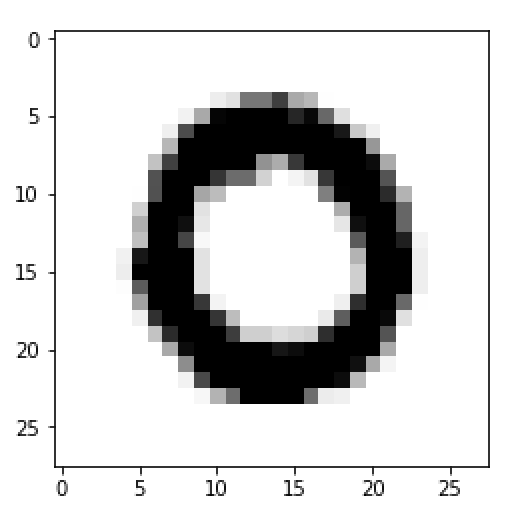
\includegraphics[width=30mm]{img/1-b/0.png}} &
      \addheight{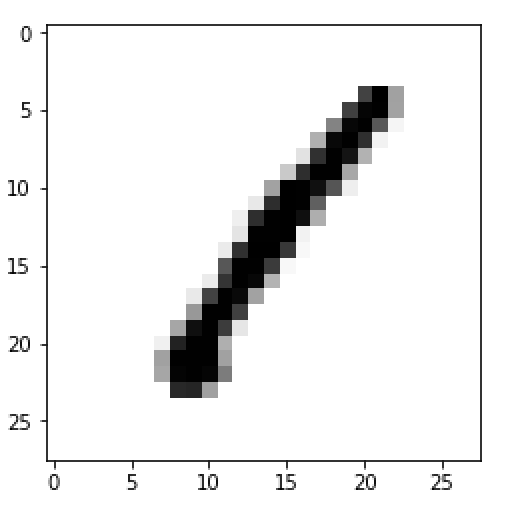
\includegraphics[width=30mm]{img/1-b/1.png}} &
      \addheight{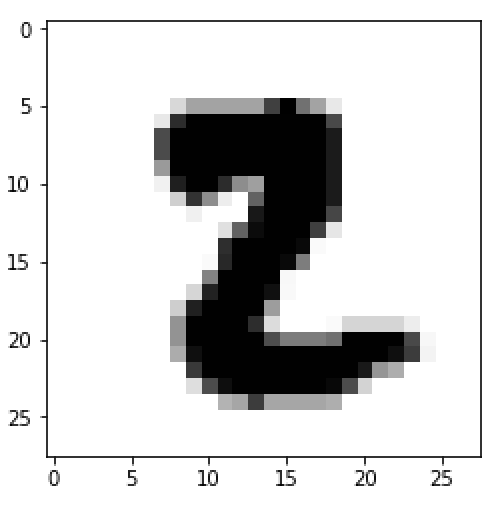
\includegraphics[width=30mm]{img/1-b/2.png}} &
      \addheight{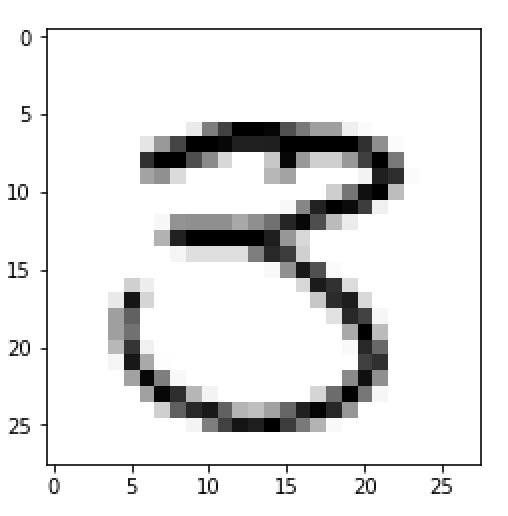
\includegraphics[width=30mm]{img/1-b/3.png}} &
      \addheight{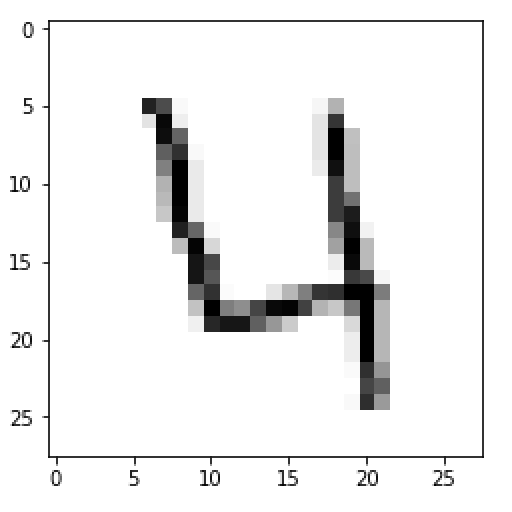
\includegraphics[width=30mm]{img/1-b/4.png}} &
      \addheight{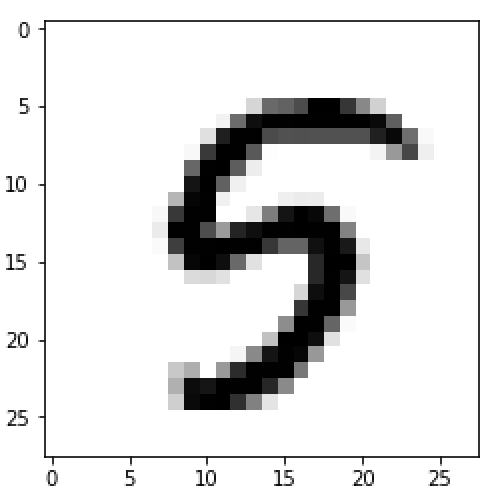
\includegraphics[width=30mm]{img/1-b/5.png}} &
      \addheight{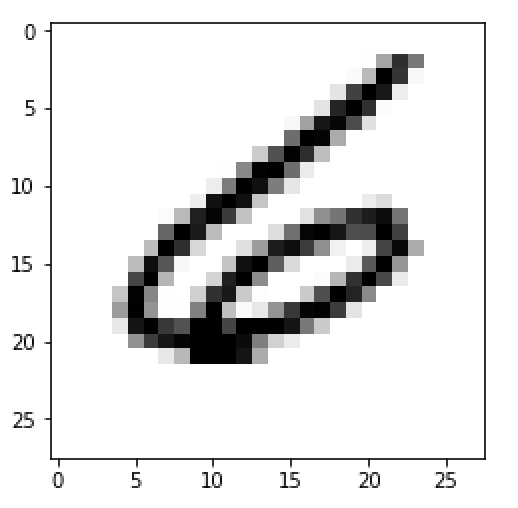
\includegraphics[width=30mm]{img/1-b/6.png}} &
      \addheight{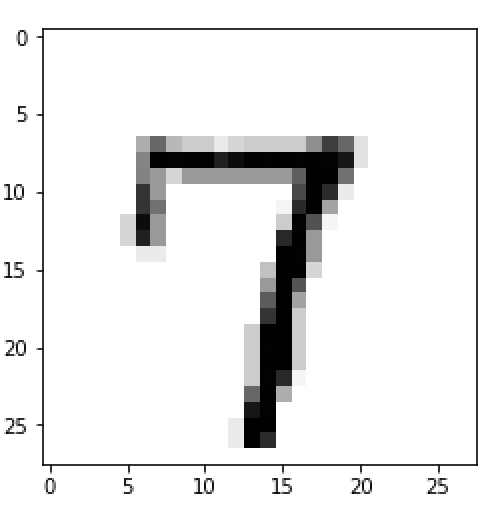
\includegraphics[width=30mm]{img/1-b/7.png}} &
      \addheight{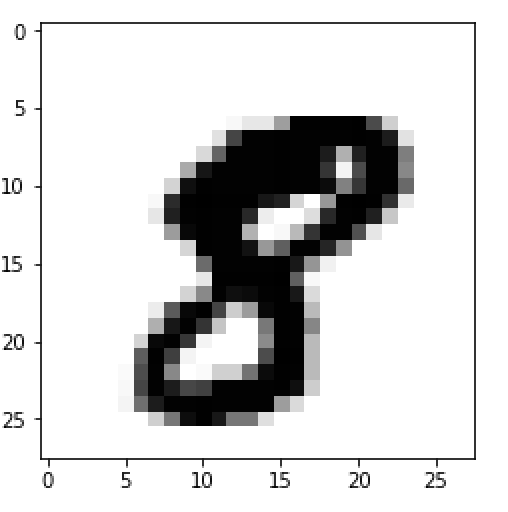
\includegraphics[width=30mm]{img/1-b/8.png}} &
      \addheight{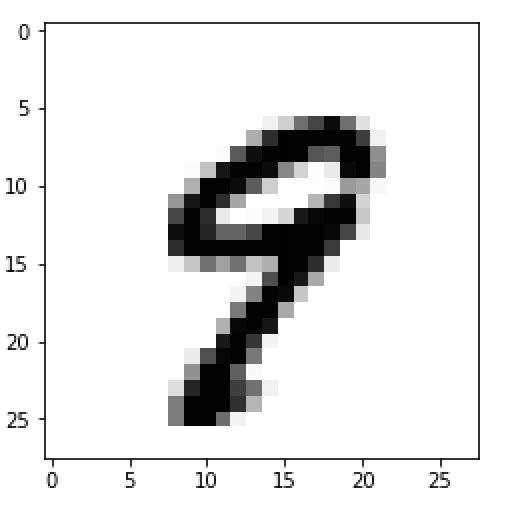
\includegraphics[width=30mm]{img/1-b/9.png}} \\
      \hline
\end{tabular}

\newpage
\subsection{c) Examine the prior probability of the classes in the training data. Is it uniform across the digits? Display a normalized histogram of digit counts. Is it even?}
To make the histogram, the only thing to do is to run a function called \textbf{displayHistogram(labels)}
Looking at the histogram below we can see that the distribution between the digits in enough uniform. We can say that is even.

\begin{figure}[ht!]
\centering
\fbox{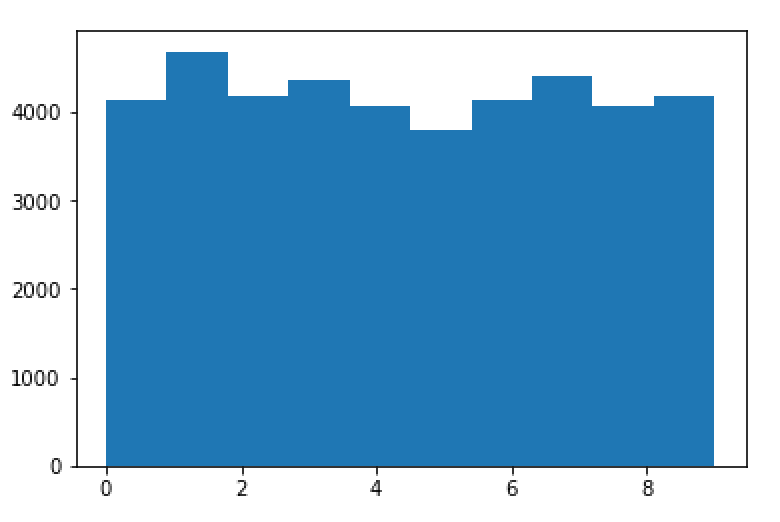
\includegraphics[scale=0.6]{img/1-c.png}}
\caption{Histogram of digit count}\label{Digit Count}
\end{figure}

\subsection{d) Pick one example of each digit from your training data. Then, for each sample digit, compute and show the best match (nearest neighbor) between your chosen sample and the rest of the training data. Use L2 distance between the two images’ pixel values as the metric. This probably won’t be perfect, so add an asterisk next to the erroneous examples (if any).}

\newpage
\section{Titulo 2}

% ============= FIN DE DOCUMENTO ==============
\end{document}

% % ················ IMAGEN ·················
% \begin{figure}[ht!]
% \centering
% \fbox{\includegraphics[scale=0.6]{img/flujo.png}}
% \caption{Flujo de caja anual}\label{flujo}
% \end{figure}
% %··········································

% % ················ IMAGEN DOBLE ·················
% \begin{figure}[ht!] \centering
% \subfloat[Esquemático]{\includegraphics[scale=0.44]{img/seguidor.png}}
% \subfloat[Simulación]{\includegraphics[scale=0.45]{img/seguidor1.png}}
% \caption{Simulación como seguidor de voltaje}\label{seguidor}
% \end{figure}
% %··········································